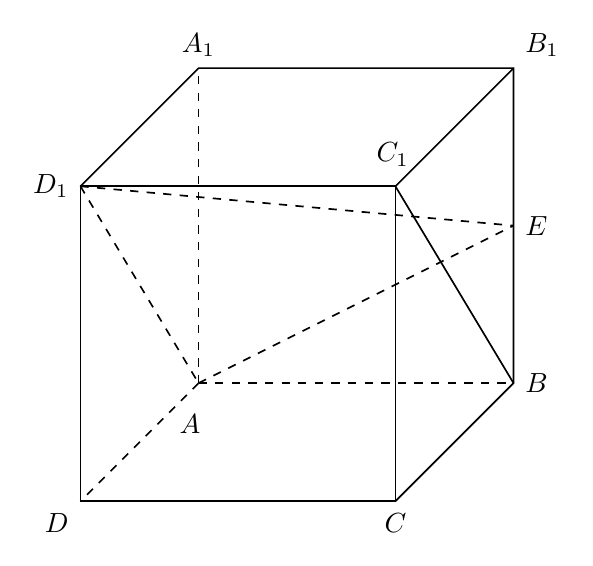
\begin{tikzpicture}[x=1cm,y=1cm,line width=.6pt,font=\normalsize,
  geometry edge/.style={solid,line width=.6pt},
  geometry label/.style={font=\normalsize,inner sep=2pt}]
\coordinate (D) at (0,0);
\coordinate (C) at (4,0);
\coordinate (A) at (1.5,1.5);
\coordinate (B) at (5.5,1.5);
\coordinate (D1) at (0,4);
\coordinate (C1) at (4,4);
\coordinate (A1) at (1.5,5.5);
\coordinate (B1) at (5.5,5.5);
\coordinate (E) at (5.5,3.5);
% solid cube + solid interior BC1
\draw[geometry edge] (D)--(C)--(C1)--(D1)--cycle;

\draw[geometry edge] (D1)--(A1)--(B1)--(B)--(C);
\draw[geometry edge] (C1)--(B1);
\draw[geometry edge] (C1)--(B);

% dashed hidden + plane AD1E
\draw[geometry edge,dashed] (A)--(B);
\draw[geometry edge,dashed] (A)--(D);
\draw[geometry edge,dashed] (A)--(A1);
\draw[geometry edge,dashed] (D1)--(A);
\draw[geometry edge,dashed] (A)--(E);
\draw[geometry edge,dashed] (D1)--(E);
% labels with clearance
\node[geometry label,above] at ([yshift=2pt]A1) {$A_{1}$};
\node[geometry label,above right] at ([xshift=2pt,yshift=2pt]B1) {$B_{1}$};
\node[geometry label,left] at ([xshift=-2pt]D1) {$D_{1}$};
\node[geometry label,above,xshift=-1pt,yshift=3pt] at ([yshift=2pt]C1) {$C_{1}$};
\node[geometry label,below left,xshift=5pt,yshift=-7pt] at ([xshift=-2pt,yshift=-2pt]A) {$A$};
\node[geometry label,right] at ([xshift=2pt]B) {$B$};
\node[geometry label,below] at ([yshift=-2pt]C) {$C$};
\node[geometry label,below left] at ([xshift=-2pt,yshift=-2pt]D) {$D$};
\node[geometry label,right] at ([xshift=2pt]E) {$E$};
\end{tikzpicture}
